% Using Unofficial UChicago CS Poster Template
% v1.1.0 released September 8, 2022
% https://github.com/k4rtik/uchicago-poster
% a fork of https://github.com/anishathalye/gemini

% COMPILE WITH: latexmk -lualatex --shell-escape main.tex
% TO CHANGE SVG TO PDF (when svg is made by draw.io and inkscape gets angry): rsvg-convert -f pdf -o data_heirarchy.pdf data_heirarchy.svg

% MOVE ACKNOWLEDMENTS BACK TO THE  RIGHT
%  FIX THE REFS TO BE ONE LINES
% WHAT IS FIO WHAT IS IOR 
% CHANGE FIRST FIGURE
% ADD CONCLUSION AND FUTURE WORK 
\documentclass[final]{beamer}

% ====================
% Packages
% ====================

\usepackage[T1]{fontenc}
\usepackage{lmodern}
% Poster Size: The conference location can accommodate posters up to 36" (height) x 48" (width).
% Height: 36 in = 91.44 cm
% Width: 48 in = 121.92 cm
\usepackage[size=custom,width=121.92,height=91.44, scale=1.0]{beamerposter}
\usetheme{gemini}
\usecolortheme{wm}
\usepackage{graphicx}
\usepackage{booktabs}
\usepackage{doi}
\usepackage[numbers]{natbib}
\usepackage[patch=none]{microtype}
\usepackage{tikz}
\usepackage{pgfplots}
\pgfplotsset{compat=1.18}
\usepackage{anyfontsize}

\usepackage{fancyvrb}
\usepackage{svg}
\usepackage{caption}
\usepackage{listings}

\pdfstringdefDisableCommands{%
\def\translate#1{#1}%
}

% ====================
% Lengths
% ====================

% If you have N columns, choose \sepwidth and \colwidth such that
% (N+1)*\sepwidth + N*\colwidth = \paperwidth
\newlength{\sepwidth}
\newlength{\colwidth}
\setlength{\sepwidth}{0.025\paperwidth}
\setlength{\colwidth}{0.3\paperwidth}

\newcommand{\separatorcolumn}{\begin{column}{\sepwidth}\end{column}}

% ====================
% Title
% ====================

\title{Benchmarking DAOS Filesystem on Aurora}

\author{Rebecca George \inst{1,2} \and Xinxin Mei \inst{2} \and Jie Ren \inst{1}}

\institute[shortinst]{\inst{1} William \& Mary \samelineand \inst{2} Jefferson Lab}

% ====================
% Footer (optional) 
% ====================

\footercontent{
  % \href{https://www.example.com}{https://www.example.com} \hfill
  CAPWIC 2026, Alexandria, Virginia \hfill
  \href{mailto:rcgeorge@wm.edu}{rcgeorge@wm.edu}}
% (can be left out to remove footer)
% 
% ====================
% Logo (optional)
% ====================

% use this to include logos on the left and/or right side of the header:
% \logoright{\includegraphics[height=7cm]{logo1.pdf}}
% \logoleft{\includegraphics[height=7cm]{logo2.pdf}}

% ====================
% Body
% ====================

\begin{document}
\addtobeamertemplate{headline}{}  
{
    \begin{tikzpicture}[remember picture,overlay]
      \node [anchor=north west, inner sep=3cm] at ([xshift=0.0cm,yshift=1.0cm]current page.north west)
      {\includegraphics[height=5.0cm]{logos/All Primary Logos/Stacked/PNG/WM_Logo_Stacked_White_Gold.png}};
      \node [anchor=north east, inner sep=3cm] at ([xshift=0.0cm,yshift=2.5cm]current page.north east)
      {\includegraphics[height=8.0cm]{logos/JLab_Logo_RGB_Red_White_Horizontal.png}};
    \end{tikzpicture}
}

\begin{frame}[t, fragile]
\begin{columns}[t]
\separatorcolumn

\begin{column}{\colwidth}

  \begin{block}{DAOS Storage System}

    Distributed Asynchronous Object Storage (DAOS) is a high performance storage 
    system using key-array-value store allowing end-to-end user space operation, 
    asynchronous I/O operation, and non-blocking I/O.


    % DAOS is provisioned to users in pools, which are persistent 
    % storage allocations spanning a set of DAOS storage 
    % engines, with a certain amount of tier 0 (Storage Class Memory (SCM)) 
    % and tier 1 (NVMe) storage. Any value or array value extent above a certain size (default=4 KiB) gets written to Tier 1, otherwise it gets written to Tier 0.

    % Users may create containers in their pool to store data. 
    % DAOS containers are logical collections of objects, 
    % which can be presented in a variety of formats, such as 
    % POSIX, HDF5, SQL Database, or PyDAOS. 
    % Containers' redundancy factor (number of replicates) may be set to some number $n$ to provide tolerance for $n$ engine failures. 
    % Containers may also be erasure coded and can use different object classes to manipulate sharding, redundancy, and erasure coding of data.
    
    \begin{figure}
      \centering
        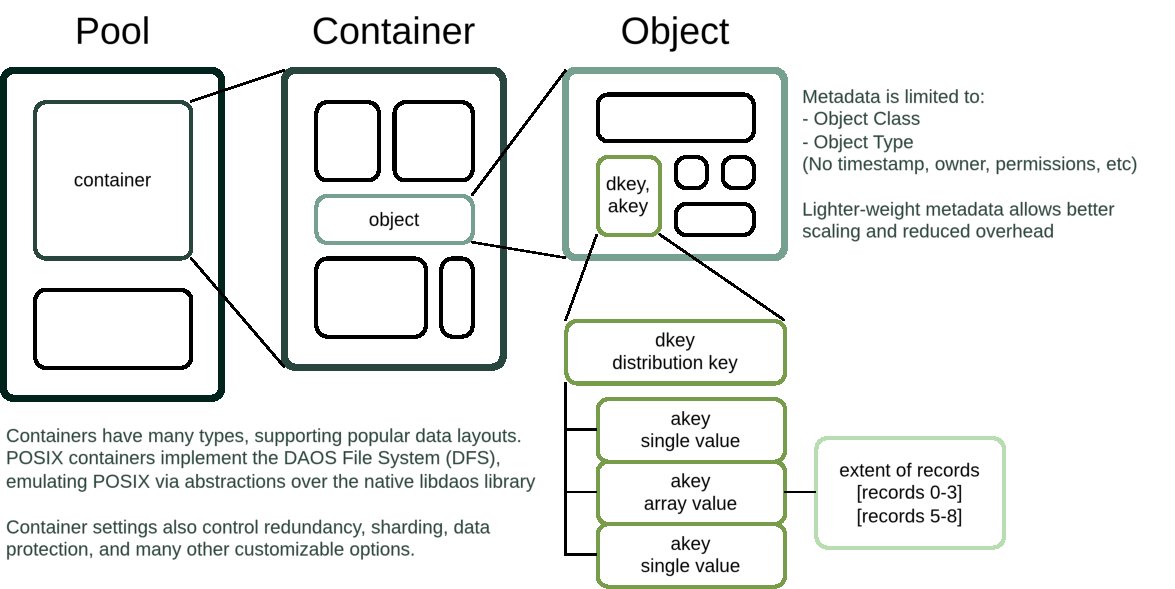
\includegraphics[width=\dimexpr 7\colwidth/8\relax]{diagrams/data_heirarchy.pdf}
      \caption{DAOS pool data hierarchy (adapted from \cite{daos_guide})}
      \label{fig:DAOS_Pool_Cont_Obj}
    \end{figure} 
    
    DAOS is provisioned in pools (storage allocations) wherein containers, 
    which are logical collections of objects (key-value stores), may be created. 
    Objects' keys have a distribution key (dkey, determining the storage target) 
    and attribute key (akey), with values of either single atomic values or arrays.

    DAOS can be accessed via the native libdaos library, 
    libpil4dfs interception library (intercepts I/O and metadata), 
    libioil interception library (intercepts I/O only), 
    and mounting a container via DFuse.
     
    % The native DAOS libary will provide the best performance, while the interception library provides the same perfromance for I/O operations without code changes.
    % Metadata operations via dfuse are slower than using the DFS API as the DFS API bypasses the kernel entirely.

    \begin{figure} 
      \centering
        \includegraphics[width=\colwidth]{diagrams/daos_arch.pdf}
        \label{fig:posix}
      \caption{DAOS client, storage, and administrative node communication. \cite{xmei_sc24} Applications on client nodes send data to/from DAOS storage nodes. Administrators may use the dmg tool and management API to communicate with the DAOS server (storage-side) and agent (client-side).}
    \end{figure}
    

  \end{block}

  \begin{block}{Aurora} 

    % \begin{figure}
    %   \centering
    %     \includegraphics{diagrams/aurora-storage-architecture.png}
    %   \caption{DAOS storage system architecture on Aurora from Argonne National Lab \cite{argonne_daos}}
    %   \label{fig:aurora-storage-architecture}
    % \end{figure}
    \begin{itemize}
      \item Argonne National Lab's Aurora supercomputer has 10,624 compute nodes with 230 PB of DAOS storage on 1024 DAOS server nodes.
      \item Aurora compute nodes have 8 HPE Slingshot-11 NICs, using dragonfly topology and use two Intel Xeon CPU Max Series, with 52 cores each. For IOR and IO500 we bind to 48 cores per node.
      \item Our pool had 127 DAOS server nodes (4064 targets, 32 targets per node) with 3 TB Tier 0 (SCM) storage and 97 TB Tier 1 (NVMe) storage. 
    \end{itemize}
  \end{block}

    \begin{block}{Benchmarking}
    We evaluated this storage system using the fio, IOR, mdtest, and IO500 I/O benchmarks. 
    We aim to characterize the I/O and metadata performance bottlenecks under a 
    variety of access patterns and client configurations on a production scale system.
    % observing effects of client-side scaling, 
    % I/O size and data transferred size, 
    % processes per node, and access type (read/write, random/sequential) 
    % on latency, IOPS, and bandwidth.
    
  \end{block}

 
\end{column}

\separatorcolumn

\begin{column}{\colwidth}




    \begin{block}{IO500}
      \par\medskip
    {IO500 is a standard high-performance computing benchmarking suite, evaluating both I/O (IOR) and metadata (mdtest) operations.}
     \par\medskip
    \renewcommand{\arraystretch}{1.4}
    \setlength{\tabcolsep}{15pt}
    \begin{minipage}[t]{0.48\colwidth}
      \centering
      {\small
      \begin{tabular}{|c|r|r|}
        \hline
        Test & \multicolumn{1}{c|}{DFS API} & \multicolumn{1}{c|}{POSIX API} \\
        \hline \hline
        ior-easy-write & 92.2 GiB/s & 81.3 GiB/s \\
        ior-easy-read & 212.6 GiB/s & 10.8 GiB/s \\
        ior-hard-write & 3.8 GiB/s & 0.7 GiB/s \\
        ior-hard-read & 15.3 GiB/s & 3.2 GiB/s \\
        \hline
        Bandwidth Score & 32.6 GiB/s & 6.5 GiB/s \\
        \hline
      \end{tabular}
      \captionof{table}{8 node IO500 bandwidth}
      }
    \end{minipage}
    \hfill
    \begin{minipage}[t]{0.48\colwidth}
      \centering
      {\small 
      \begin{tabular}{|c|r|r|}
        \hline
        Test & \multicolumn{1}{c|}{DFS API} & \multicolumn{1}{c|}{POSIX API} \\
        \hline \hline
        find & 775.6 kIOPS & 1.6 kIOPS \\
        mdtest-easy-write & 219.4 kIOPS & 4.0 kIOPS \\
        mdtest-hard-write & 60.6 kIOPS & 1.1 kIOPS \\
        mdtest-hard-read & 807.3 kIOPS & 3.9 kIOPS \\
        mdtest-easy-stat & 1112.2 kIOPS & 4.0 kIOPS \\
        mdtest-hard-stat & 1098.3 kIOPS & 3.9 kIOPS \\
        mdtest-easy-delete & 301.0 kIOPS & 3.4 kIOPS \\
        mdtest-hard-delete & 302.6 kIOPS & 0.4 kIOPS \\
        \hline
        IOPS Score & 417.7 kIOPS  & 2.2 kIOPS \\
        \hline
      \end{tabular}
      \captionof{table}{8 node IO500 IOPS} 
      % rounded to 1 decimal point
      }
    \end{minipage}
    \par\medskip
    {{\normalsize{\textbf{DFS API achieved \approx5x higher bandwidths and \approx190x higher IOPS than POSIX API on a DFuse mounted POSIX container, making major improvements to metadata and reading operations}}}}
    
  \end{block}

  \begin{block}{DFuse POSIX Bandwidth}

    
    
    \begin{figure}
      \centering
        \includesvg[width=\colwidth]{diagrams/fio_bw_vs_bs_hueRW_nj-16_iod-16.svg} 
      \caption{Single client bandwidth vs block size (I/O unit size) for fio using pvsync I/O engine.}
      \label{fig:fio_bw_vs_bs_hueRW_nj-16_iod-16}
    \end{figure}
    \normalsize{
    \begin{itemize}
      \item \textbf{DFuse POSIX bandwidth increased with I/O unit size, saturating at I/O unit size of 1-2 MiB}
      \item Workloads with more writing, relative to reading, achieved higher throughput via DFuse
      \item Random vs sequential access had little effect on throughput
      % \item Unbuffered I/O has generally higher throughput than buffered I/O
      % \item Increasing the number of fio jobs %(additional threads cloning the original thread) 
      % increases latency, but has little effect on IOPS or bandwidth % omitting because I believe this must have been all single core binding due to the strange core affinity issues
      % \item The number of I/O units kept in flight has little effect on latency, bandwidth, or IOPS
    \end{itemize}
    }
    % This desmonstrates the 
      % performance achieved by POSIX container access via dfuse mount points. 
      % pvsync I/O engine uses vectorized system calls and allows read/write 
      % from non-contiguous buffers.
    % \begin{figure} 
    %   \centering
    %     \includesvg[width=\colwidth]{diagrams/bw_stacked_combined.svg} 
    %   % Read is reading only, 4:1 is 4 reads per write, 1:1 is an equal amount of reading and writing, 1:4 is 1 read per 4 writes, and write is writing only.
    %   \caption{
    %   For one client node with 16 jobs, 16 I/O units kept in flight, and a block size of 1 MiB, 
    %   the proportions of overall bandwidth spent reading and writing for buffered and unbuffered workloads.
    %   The yellow line indicates the expected ratio of reading vs writing.
    %   } 
    %   \label{fig:bw_stacked_combined}
    % \end{figure} 
    % \textcolor{wmgreen}{\large{\textbf{Read and write proportions of throughput are approximately proportional to the amount of reading or writing done.}}}
    

    % across different workloads is reflect approximately the amount of reading and writing done. 

    % Buffered I/O will use an intermediate buffer between applications 
    %   (fio) and system calls to preadv*/pwritev*, while unbuffered I/O will 
    %   go straight to system calls. 

    
  \end{block}


  \begin{block}{IOR Latency}
    \begin{figure} 
      \centering 
      \includesvg[width=\colwidth]{diagrams/ior_latency.svg} 
      \caption{For a transfer size of 1 MiB, the IOR latency vs number of tasks, using DFS API.}
      % For <8 nodes, the write latency stays relatively constant as the number of 
      % tasks increases, but larger numbers of nodes accrue more latency as the 
      % number of tasks increases. Read latency ellicited a <10 ms increase in 
      % latency as more tasks were used, but all test cases stayed under 20 ms latency 
      % (10 ms difference from 1 task) except the largest number of nodes used (32). 
    \label{fig:ior_latency}
    \end{figure}
    {{\normalsize{\textbf{DFS I/O latency increased with more tasks and nodes, with greater effects on writing than reading}}}}
  \end{block}
 

\end{column}

\separatorcolumn

\begin{column}{\colwidth}

  \begin{block}{IOR Bandwidth}

    \begin{figure}
      \centering
        \includesvg[width=\colwidth]{diagrams/ior_bw-vs-tasks_hue-nodes-2M.svg} 
      \caption{For a transfer size (I/O unit size) of 2 MiB, the IOR bandwidth vs number of tasks, using the DFS API}
      \label{fig:ior_bw-vs-tasks_hue-nodes_2M}
    \end{figure}
    \begin{figure}
      \centering
        \includesvg[width=\colwidth]{diagrams/ior_bw-vs-tasks_hue-nodes_16M.svg} 
      \caption{For a transfer size (I/O unit size) of 16 MiB, the IOR bandwidth vs number of tasks, using the DFS API.}
      \label{fig:ior_bw-vs-tasks_hue-nodes_16M}
    \end{figure}
    \normalsize{
    \begin{itemize}
      \item \textbf{Read and write bandwidth increased with as tasks increased, saturating around 32 tasks}
      \item \textbf{At high task counts, sufficiently large transfer sizes reduce read bandwidth}
    \end{itemize}
    }
    % With a large transfer size, we see that reading with more than 
    % 8 or 16 tasks per node decreases bandwidth dramatically, 
    % although smaller numbers of tasks provide higher bandwidth 
    % than the same number of tasks run with a smaller transfer size. 
    % A small transfer size, such as 16 KiB provided relatively lower bandwidths 
    % than either 1-2 MiB or 16 MiB, due to having to make many small I/O operations. 
    % Reading has similar throughput to writing using the native DFS API, 
    % until the number of nodes used become larger, when it surpassed write bandwidth.


    \begin{figure}
      \centering
        \includesvg[width=\dimexpr 3\colwidth/4\relax]{diagrams/ior_bw-vs-tx_8ppn.svg} 
      \caption{For 8 tasks per node, the IOR bandwidth vs number of tasks, using the DFS API.}
    \end{figure}
    \normalsize{
    \begin{itemize}
      \item \textbf{For a single client, reading is slightly more performant than writing across transfer sizes}
      \item Sufficiently small transfer sizes (16 KiB) provide low throughput, both for a single client (Figure 7) and all numbers of nodes and tasks per node tested
    \end{itemize}
    }
    % As with the pvsync I/O engine, 
    % the DFS API begins to saturate at transfer sizes above 1-2 MiB. 
    % The same transfer sizes, however, provide 2-3x higher bandwidth 
    % for single-client workloads. Unlike the non-native API, 
    % we see read bandwidths are on a similar scale to write bandwidth 
    % and are higher overall, instead of being dramatically lower 
    % than write bandwidths.
    
 
  \end{block}

    \begin{block}{Acknowledgments}
  This research used resources of the Argonne Leadership Computing Facility, 
  which is a U.S. Department of Energy Office of Science User Facility 
  operated under contract DE-AC02-06CH11357. This work was supported by NSF OAC-2348350.
  \end{block}
  

  \begin{block}{References} 

    \nocite{*}
    \footnotesize{\bibliographystyle{plainnat}\bibliography{poster}}
 
  \end{block}

\end{column}

\separatorcolumn
\end{columns}
\end{frame}

\end{document}